
\documentclass[11pt,a4paper,openany]{report}
\usepackage[T1]{fontenc}
\usepackage[utf8]{inputenc}
\usepackage{lmodern}
\usepackage{microtype}
\usepackage{amsmath,amssymb,amsthm,mathtools,bm}
\usepackage{booktabs,array,longtable,tabularx}
\usepackage{xcolor}
\usepackage[margin=22mm,headheight=23pt]{geometry}
\usepackage{enumitem}
\usepackage{fancyhdr}
\usepackage{fancyvrb}
\usepackage{graphicx}
\usepackage{url}
\usepackage{xurl}
\usepackage{hyperref}
\definecolor{finblue}{HTML}{1F5A99}
\definecolor{fingreen}{HTML}{19733A}
\definecolor{finorange}{HTML}{D55E00}
\definecolor{finred}{HTML}{A61B1B}
\definecolor{finviolet}{HTML}{6A3D9A}
\definecolor{fingray}{HTML}{4D4D4D}

\hypersetup{unicode=true,colorlinks=true,linkcolor=finblue,citecolor=fingreen,
urlcolor=finblue,pdftitle={FIN Local Research Checkpoint P465--P469},
pdfauthor={Krzysztof Żuchowski},
pdfsubject={Strict full-simplex uniqueness and a support-ladder rational dual certificate},
pdfkeywords={FIN, strict symmetrization, equality cases, quantum comb, semidefinite duality, KKT, rational certificate}}
\pagestyle{fancy}\fancyhf{}
\fancyhead[L]{\small FIN Checkpoint P465--P469}
\fancyhead[R]{\small Release 10.43}\fancyfoot[C]{\thepage}

\setlength{\parindent}{0pt}
\setlength{\parskip}{0.55em}
\setlist{nosep,leftmargin=2em}
\setcounter{tocdepth}{2}
\setcounter{secnumdepth}{3}
\emergencystretch=3em
\newcommand{\one}{\bm 1}
\newcommand{\C}{\mathbb C}
\newcommand{\R}{\mathbb R}
\newcommand{\Z}{\mathbb Z}
\newcommand{\statusProven}{\textcolor{fingreen}{[Proven]}}
\newcommand{\statusStrong}{\textcolor{finblue}{[Strong evidence]}}
\newcommand{\statusModerate}{\textcolor{finviolet}{[Moderate evidence]}}
\newcommand{\statusWeak}{\textcolor{fingray}{[Weak evidence]}}
\newcommand{\statusSpeculative}{\textcolor{finorange}{[Speculative]}}
\newcommand{\statusRefuted}{\textcolor{finred}{[Refuted]}}

\begin{document}\hypersetup{pageanchor=false}
\begin{titlepage}\centering\vspace*{8mm}
{\Large\bfseries FIN Local Research --- Release 10.43\par}\vspace{10mm}
{\Huge\bfseries Checkpoint P465--P469\par}\vspace{6mm}
{\Large Strict Full-Simplex Uniqueness and a Support-Ladder\
Rational Dual Certificate\par}\vspace{14mm}
{\Large Krzysztof \.Zuchowski\par}\vspace{2mm}
{\normalsize Independent Researcher --- Fractal Information Theory Project\par}
{\normalsize ORCID: 0009-0002-0909-3613\par}\vspace{8mm}
{\large 1 August 2026\par}{\normalsize Publication --- Preprint; Version 1.0.0\par}
\vfill
\begin{minipage}{0.92\textwidth}\small
\textbf{Central results.} Reversal symmetrization is proved strict outside
the palindromic fixed set, closing full-simplex uniqueness for the declared
coarse-erasure model. A new exact-rational nested dual proves
\[
0.52332810026048937\le D_3^{\rm global}\le0.52332810067104088,
\]
with exact gap $4.1055151\times10^{-10}$.

\medskip\textbf{Localized frontier.} The canonical O167 support ladder
satisfies the complete floating KKT residual to $1.33\times10^{-15}$, but an
exact interval root and exact attainment remain open.

\medskip\textbf{Boundary.} No selector, dimensional source, laboratory
record, complete legacy--strict bridge, role transfer, full physical closure,
or Theory of Everything is claimed.

\medskip\textbf{License.} CC BY 4.0.
\end{minipage}\vfill\end{titlepage}
\hypersetup{pageanchor=true}\pagenumbering{roman}
\chapter*{Publication statement}\addcontentsline{toc}{chapter}{Publication statement}
This monograph reports local analytical and computer-assisted Programs P465,
P468, and P469. It uses no laboratory record, external audit, internet result,
remote computation, or physical validation.
\tableofcontents\clearpage\pagenumbering{arabic}

\chapter{Executive summary}

This checkpoint completes local Programs P465, P468, and P469. It uses exact algebra, rational arithmetic, exact Sylvester tests, certified trigonometric enclosures, finite-dimensional semidefinite duality, and deterministic local numerical computation. It uses no internet result, laboratory record, external audit, remote computation, or empirical physical evidence.

The principal results are as follows.

\begin{enumerate}
\item 
\textbf{P465 --- \statusProven{}.} The equality cases of the P452 reversal symmetrization theorem are classified. For the declared three-use coarse erasure objective, reversal averaging is strict at every non-palindromic point of the complete four-sector probability simplex. Combined with the P458 strict-curvature theorem, this proves that the full-simplex maximizer is unique and has the form

\[
   p_*=(a_*,\tfrac12-a_*,\tfrac12-a_*,a_*),
   \]

where

\[
   0.2276921883225489
   \le a_*\le
   0.22769218832267057.
   \]

The interval width is below \(1.22\times10^{-13}\). This is uniqueness in the complete declared four-sector simplex, not merely uniqueness among palindromic representatives.

\item 
\textbf{P469 --- \statusStrong{}, with an exact necessity theorem.} For a positive interior normalizer \(N\), the canonical trace-norm support is

\[
   X_3(N)=\frac12N^{-1/2}
   \left|N^{1/2}\Delta N^{1/2}\right|N^{-1/2}.
   \]

Complementary slackness proves that an interior optimal ordered comb must make the two principal blocks agree at every lower causal level. Solving those necessary equations on the O167 face gives

\[
   (A,B,u)\approx
   (0.2871664153717576,
    0.06877721090495502,
    0.009493709596691087),
   \]

with full residual infinity norm

\[
   1.3322676295501878\times10^{-15}.
   \]

The normalizer is safely interior, with minimum eigenvalue \(0.057723558496969855\), and the transformed process difference is nonsingular, with minimum absolute eigenvalue \(0.008009754936339366\). The numerical result is compelling but does not prove an exact nonlinear root.

\item 
\textbf{P468 --- \textcolor{fingreen}{[Computer-assisted proof]}.} The P469 support ladder is shifted by explicit positive margins, rounded to rational matrices, and admitted only after exact positivity verification. The new global three-slot ordered-comb bracket is

\[
   0.52332810026048937
   \le D_3^{\rm global}\le
   0.52332810067104088.
   \]

Its exact width is

\[
   \frac{41055151}{10^{17}}
   =4.1055151\times10^{-10},
   \]

approximately \(535.8902\) times narrower than the Release-10.42 bracket. The smallest accepted certified slack lower bound is \(9.9996948523231345\times10^{-12}>0\).

\end{enumerate}

The new theoretical objects are O176 Strict Reversal Equality Isolator, O177 Interior Comb Support Ladder, and O178 Support-Ladder Rational Closure Tube.

The results do not prove exact O167 attainment, uniqueness of the full ordered-comb optimizer, a FIN selector, a dimensional source, a physical preparation or instrument, a laboratory record, a complete legacy-to-strict kernel bridge, role transfer, \(L_{\rm total}\), Standard Model or gravity closure, or a Theory of Everything.

\chapter{Confidence convention}

\begin{center}
\begingroup\small
\setlength{\tabcolsep}{2.5pt}
\renewcommand{\arraystretch}{1.16}
\begin{longtable}{@{}p{0.420\textwidth}p{0.420\textwidth}@{}}
\toprule
\textbf{Label} & \textbf{Meaning} \\
\midrule
\endhead
\statusProven{} & Exact analytic or finite algebraic consequence of the declared premises \\
\textcolor{fingreen}{[Computer-assisted proof]} & Finite rational or outward-interval certificate with auditable artifacts \\
\statusStrong{} & Reproducible numerical evidence lacking a complete exact certificate \\
\textcolor{finviolet}{[Conditional]} & Conclusion dependent on an explicitly supplied mathematical interface \\
\textcolor{finorange}{[Open]} & Current local artifacts do not decide the proposition \\
\statusRefuted{} & A stated candidate or route fails a rigorous necessary test \\
\textcolor{finred}{[Blocked by external evidence]} & Laboratory, calibration, custody, or an external record is indispensable \\
\bottomrule
\end{longtable}
\endgroup
\end{center}

\chapter{State map and non-promotion guardrails}

\begin{center}
\begingroup\small
\setlength{\tabcolsep}{2.5pt}
\renewcommand{\arraystretch}{1.16}
\begin{longtable}{@{}p{0.237\textwidth}p{0.323\textwidth}p{0.300\textwidth}@{}}
\toprule
\textbf{Lane} & \textbf{Release 10.42 state} & \textbf{Release 10.43 state} \\
\midrule
\endhead
Declared coarse-erasure maximizer & Unique palindromic representative; asymmetric co-optimizers open & Unique on the complete declared four-sector simplex \\
Maximizer location & Width below \(1.22\times10^{-13}\) & Unchanged and now full-simplex licensed \\
Three-slot global full cone & Gap \(2.2001054063\times10^{-7}\) & Gap \(4.1055151\times10^{-10}\) \\
O167 full-cone stationarity & Open & Full KKT residual \(1.33\times10^{-15}\), strong evidence only \\
Exact O167 attainment & Open & Open: exact nonlinear root not isolated \\
Full-cone optimizer uniqueness & Open & Open \\
Selector /\allowbreak{} QW-2191 & Open & Unchanged \\
Dimensional source & Missing & Unchanged \\
Laboratory evidence & None & None \\
Legacy-to-strict bridge & Incomplete & Unchanged \\
\bottomrule
\end{longtable}
\endgroup
\end{center}

The intermediate and strict kernels remain distinct:

\[
K_{\rm legacy,ont}(d)=
\frac{\alpha_{\rm geo}\cos(\omega d+\phi)}
{1+\beta_{\rm tors}d},
\qquad
K_{\rm strict,gate}(d)=
\frac{\cos(\omega d+\phi)}{1+\beta d^\eta}.
\]

No result below silently substitutes one kernel for the other. These programs are downstream finite operational calculations and derive neither kernel. They transfer no legacy physical role. The ontology remains

\[
\text{nadsoliton}\longrightarrow\text{light}\longrightarrow
\text{matter}\longrightarrow\text{emergent observer},
\]

with no informational layer underneath the nadsoliton.

\chapter{P465 --- strict equality in reversal symmetrization}

\section{Question left open by P458}

Let

\[
p=(p_0,p_1,p_2,p_3),\qquad p_i\ge0,\qquad\sum_i p_i=1,
\]

and let reversal be

\[
Rp=(p_3,p_2,p_1,p_0).
\]

P452 proved that the declared coarse-erasure objective \(F\) obeys

\[
F\!\left(\frac{p+Rp}{2}\right)\ge F(p).
\]

P458 then proved that the palindromic branch contains exactly one maximizer. Those two results alone did not exclude an asymmetric point satisfying equality under symmetrization. P465 asks for the complete equality set.

\section{Square-root coordinates}

Write

\[
(x,y,z,w)=(\sqrt{p_0},\sqrt{p_1},\sqrt{p_2},\sqrt{p_3}).
\]

Introduce the pair radii and angles

\[
x=\sqrt2X\cos\alpha,\qquad
w=\sqrt2X\sin\alpha,
\]

\[
y=\sqrt2Y\cos\beta,\qquad
z=\sqrt2Y\sin\beta,
\]

with \(X,Y\ge0\) and \(\alpha,\beta\in[0,\pi/2]\). Reversal averaging replaces both endpoint square-root masses by \(X\) and both middle square-root masses by \(Y\).

Only the two-survivor sector requires the nontrivial P452 coefficient analysis. Put

\[
q=\frac45,\qquad \theta=\frac{2\pi}{15},\qquad
\kappa=4q^2\cos^2\theta.
\]

Exact rational trigonometric enclosure gives

\[
\kappa-1\ge1.1364871761393385>0.
\]

\section{Exact defect factorization}

For \(Y>0\), put \(r=X/Y\). Direct block reduction gives

\[
D_2(\operatorname{sym}p)^2-D_2(p)^2
=16q^2\sin^2\theta\,Y^4
\left(c_0+c_1r+c_2r^2\right),
\]

where

\[
c_0=\frac{\cos^2(2\beta)}9,
\]

\[
c_1=\frac{2\sqrt3}{9}
\left[1-\sin(2\beta)\cos(\alpha-\beta)\right],
\]

and

\[
c_2=
\frac{-\cos(2\alpha)\cos(2\beta)
+\kappa\cos^2(\alpha+\beta)}3.
\]

The key exact trigonometric identity is

\[
\cos^2(\alpha+\beta)-
\cos(2\alpha)\cos(2\beta)
=\sin^2(\alpha-\beta).
\]

It converts the quadratic coefficient into the explicit sum

\[
\boxed{
c_2=\frac{(\kappa-1)\cos^2(\alpha+\beta)
+\sin^2(\alpha-\beta)}3.}
\]

All three coefficients are nonnegative on the declared angle square. Because \(\kappa-1>0\),

\[
c_2=0
\quad\Longleftrightarrow\quad
\cos(\alpha+\beta)=0
\ \text{and}\ 
\sin(\alpha-\beta)=0.
\]

Within \([0,\pi/2]^2\), this is equivalent to

\[
\alpha=\beta=\frac\pi4.
\]

Thus for \(X,Y>0\), equality forces \(x=w\) and \(y=z\).

\section{Boundary faces}

The angular argument must not silently divide by a vanishing pair radius. Both singular faces are treated separately.

If \(X=0<Y\), then \(r=0\) and the defect reduces to its constant term. Equality means

\[
c_0=0\quad\Longleftrightarrow\quad\beta=\frac\pi4.
\]

Hence \(x=w=0\) and \(y=z\): the point is palindromic.

If \(Y=0<X\), the two-survivor sector is identically blind to endpoint imbalance. This is the exceptional face that a proof using only \(D_2\) would miss. The three-survivor block instead gives the exact gain

\[
D_3(\operatorname{sym}p)-D_3(p)
=q^3\sin(3\theta)(x-w)^2.
\]

Since \(q>0\) and \(0<3\theta<\pi\), equality holds exactly when \(x=w\). The impossible case \(X=Y=0\) is excluded by normalization.

\section{Theorem}

\textbf{Strict reversal theorem. \statusProven{}} For the exact declared three-use, permutation-symmetric Hamming-sector code, \(q=4/5\), \(\theta=2\pi/15\), and its heralded-loss objective,

\[
F\!\left(\frac{p+Rp}{2}\right)=F(p)
\quad\Longleftrightarrow\quad Rp=p.
\]

Combining this theorem with P458 gives a unique maximizer on the complete declared four-sector simplex. The theorem does not extend automatically to adaptive inputs, another code, another channel, or an unheralded-loss model.

\section{Falsification checks}

A deterministic scan checked 4,098 non-palindromic points, including both singular faces and 4,096 Dirichlet points. Every observed objective gain was positive; the smallest was \(3.776242863018364\times10^{-6}\). These samples are not used as the proof. Their role is to detect implementation or sign errors in the exact derivation.

\chapter{P469 --- the interior comb support ladder}

\section{Primal and dual setting}

The three-slot primal semidefinite program is

\[
\begin{aligned}
\text{maximize}\quad&
\frac12\operatorname{Tr}[\Delta(T_+-T_-)]\\
\text{subject to}\quad&
T_++T_-=B_0\oplus B_1,\\
&B_0+B_1=C_0\oplus C_1,\\
&C_0+C_1=\operatorname{diag}(d_0,d_1),\\
&d_0+d_1=1,
\end{aligned}
\]

with all primal variables positive. Its dual minimizes \(\lambda\) under

\[
X_3\succeq\pm\frac\Delta2,
\]

\[
X_2\succeq(X_3)_{00},\quad
X_2\succeq(X_3)_{11},
\]

\[
X_1\succeq(X_2)_{00},\quad
X_1\succeq(X_2)_{11},
\]

\[
\lambda\ge(X_1)_{00},\qquad
\lambda\ge(X_1)_{11}.
\]

Finite-dimensional Slater duality applies.

\section{Canonical support operator}

For a fixed positive normalizer \(N=T_++T_-\), define

\[
H=N^{1/2}\Delta N^{1/2}.
\]

If \(H\) is nonsingular, the positive and negative spectral projectors \(P_+\), \(P_-\) give the Helstrom testers

\[
T_\pm=N^{1/2}P_\pm N^{1/2}.
\]

The associated top dual support is

\[
\boxed{
X_3(N)=\frac12N^{-1/2}|H|N^{-1/2}.}
\]

It obeys

\[
X_3\succeq\pm\frac\Delta2
\]

and the top complementary contacts vanish:

\[
\operatorname{Tr}\!\bigl[
(X_3-\Delta/2)T_+\bigr]=0,
\qquad
\operatorname{Tr}\!\bigl[
(X_3+\Delta/2)T_-\bigr]=0.
\]

This is not a fitted dual matrix. It is the canonical supporting operator of the trace norm at the supplied interior normalizer.

\section{Interior cascade necessity theorem}

At the O167 candidate, \(B_0,B_1,C_0,C_1\) are positive definite and \(d_0,d_1>0\). If this candidate is globally optimal, complementary slackness forces

\[
X_2-(X_3)_{00}=0,
\qquad
X_2-(X_3)_{11}=0,
\]

\[
X_1-(X_2)_{00}=0,
\qquad
X_1-(X_2)_{11}=0,
\]

and

\[
\lambda-(X_1)_{00}=0,
\qquad
\lambda-(X_1)_{11}=0.
\]

The reason is elementary and exact: if \(S\succeq0\), \(P\succ0\), and \(\operatorname{Tr}(SP)=0\), then \(S=0\). Therefore the support matrix must have equal inherited blocks at every causal level. These equations test full ordered-comb stationarity, not only stationarity inside the three-dimensional O167 face.

\section{Numerical root and robustness}

The least-squares root is

\[
(A,B,u)=
(0.2871664153717576,
0.06877721090495502,
0.009493709596691087).
\]

The measured residuals are

\begin{center}
\begingroup\small
\setlength{\tabcolsep}{2.5pt}
\renewcommand{\arraystretch}{1.16}
\begin{longtable}{@{}p{0.420\textwidth}p{0.420\textwidth}@{}}
\toprule
\textbf{Equation level} & \textbf{Residual} \\
\midrule
\endhead
\(X_3^{00}-X_3^{11}\), Frobenius & \(2.408655631223323\times10^{-15}\) \\
\(X_2^{00}-X_2^{11}\), Frobenius & \(1.546375975750693\times10^{-15}\) \\
\((X_1)_{00}-(X_1)_{11}\) & \(2.220446049250313\times10^{-16}\) \\
Full residual, infinity norm & \(1.3322676295501878\times10^{-15}\) \\
Maximum absolute trace contact & \(4.198098375228894\times10^{-16}\) \\
\bottomrule
\end{longtable}
\endgroup
\end{center}

Two separation checks make accidental nondifferentiability implausible:

\[
\lambda_{\min}(N)=0.057723558496969855>0,
\]

\[
\min_j|\lambda_j(H)|=0.008009754936339366>0.
\]

The numerical primal value is \(0.5233281002710412\). The constructed support scalar differs only at binary64 roundoff. The reported negative signed difference of about \(4.4\times10^{-16}\) is not interpreted as a duality violation because the averaged floating ladder is not an exact feasible dual.

\section{Why P469 is not yet a theorem of attainment}

A residual of \(10^{-15}\) does not prove a real zero. The map contains matrix square roots and the matrix absolute value. Exact closure requires an outward enclosure of this matrix functional calculus, an invertible interval Jacobian, and an interval Newton or Krawczyk inclusion showing that one exact root lies inside a stated box. Until that certificate exists, exact O167 attainment and full-cone uniqueness remain open.

\chapter{P468 --- exact rational support-ladder upper bound}

\section{Construction}

P468 turns the P469 locator into a proof-grade dual without promoting the floating root. Starting from \(X_3(N)\), each causal level receives a positive identity shift:

\[
\widetilde X_3=X_3+\varepsilon I_8,
\]

\[
\widetilde X_2=\frac12
\left[(\widetilde X_3)_{00}+(\widetilde X_3)_{11}\right]
+\varepsilon I_4,
\]

\[
\widetilde X_1=\frac12
\left[(\widetilde X_2)_{00}+(\widetilde X_2)_{11}\right]
+\varepsilon I_2,
\]

\[
\widetilde\lambda=
\max_i(\widetilde X_1)_{ii}+\varepsilon.
\]

Three shifts were attempted: \(10^{-9}\), \(3\times10^{-10}\), and \(10^{-10}\). Every floating candidate remained only a proposal until exact rational admission.

\section{Rationalization and exact positivity}

The best accepted candidate uses \(\varepsilon=10^{-10}\) and denominator \(10^{17}\). Its rational upper value is

\[
\widetilde\lambda_{\mathbb Q}
=\frac{6541601258388011}{12500000000000000}
=0.52332810067104088.
\]

All six matrix slacks were shifted by candidate rational margins and tested by exact leading principal minors. The two scalar slacks were checked exactly. For the two trigonometric top slacks, the inherited rational midpoint has maximum entry radius

\[
3.8143459608252896\times10^{-17},
\]

and the full operator perturbation payment is

\[
3.0514767686602317\times10^{-16}.
\]

The accepted slack summary is:

\begin{center}
\begingroup\small
\setlength{\tabcolsep}{2.5pt}
\renewcommand{\arraystretch}{1.16}
\begin{longtable}{@{}p{0.420\textwidth}p{0.420\textwidth}@{}}
\toprule
\textbf{Dual slack} & \textbf{Certified lower bound} \\
\midrule
\endhead
\(X_3+\Delta/2\) & \(9.9996948523231345\times10^{-12}\) \\
\(X_3-\Delta/2\) & \(9.9996948523231345\times10^{-12}\) \\
\(X_2-(X_3)_{00}\) & \(10^{-11}\) \\
\(X_2-(X_3)_{11}\) & \(10^{-11}\) \\
\(X_1-(X_2)_{00}\) & \(10^{-11}\) \\
\(X_1-(X_2)_{11}\) & \(10^{-10}\) \\
\(\lambda-(X_1)_{00}\) & \(10^{-10}\) \\
\(\lambda-(X_1)_{11}\) & \(1.0000024\times10^{-10}\) \\
\bottomrule
\end{longtable}
\endgroup
\end{center}

All are strictly positive. Thus weak duality licenses the upper bound independently of whether the P469 floating root is exact.

\section{Global bracket}

Combining the accepted dual with the inherited exact lower certificate gives

\[
\boxed{
0.52332810026048937
\le D_3^{\rm global}\le
0.52332810067104088.}
\]

The exact gap is

\[
\boxed{
\frac{41055151}{10^{17}}
=4.1055151\times10^{-10}.}
\]

Relative to P464, the certified gap is reduced by a factor of \(535.8902239331674\). Relative to P454, it is reduced by more than four orders of magnitude.

The corresponding global success probability obeys

\[
0.761664050130244685
\le p_{\rm succ}^{\rm global}\le
0.76166405033552044.
\]

\section{Scope}

The strict positive shifts deliberately prevent exact complementarity. P468 is an exact global value bracket, not a theorem that O167 attains the optimum. It also does not show optimizer uniqueness. A positive gap cannot be rounded away, irrespective of its smallness.

\begin{figure}[htbp]
\centering
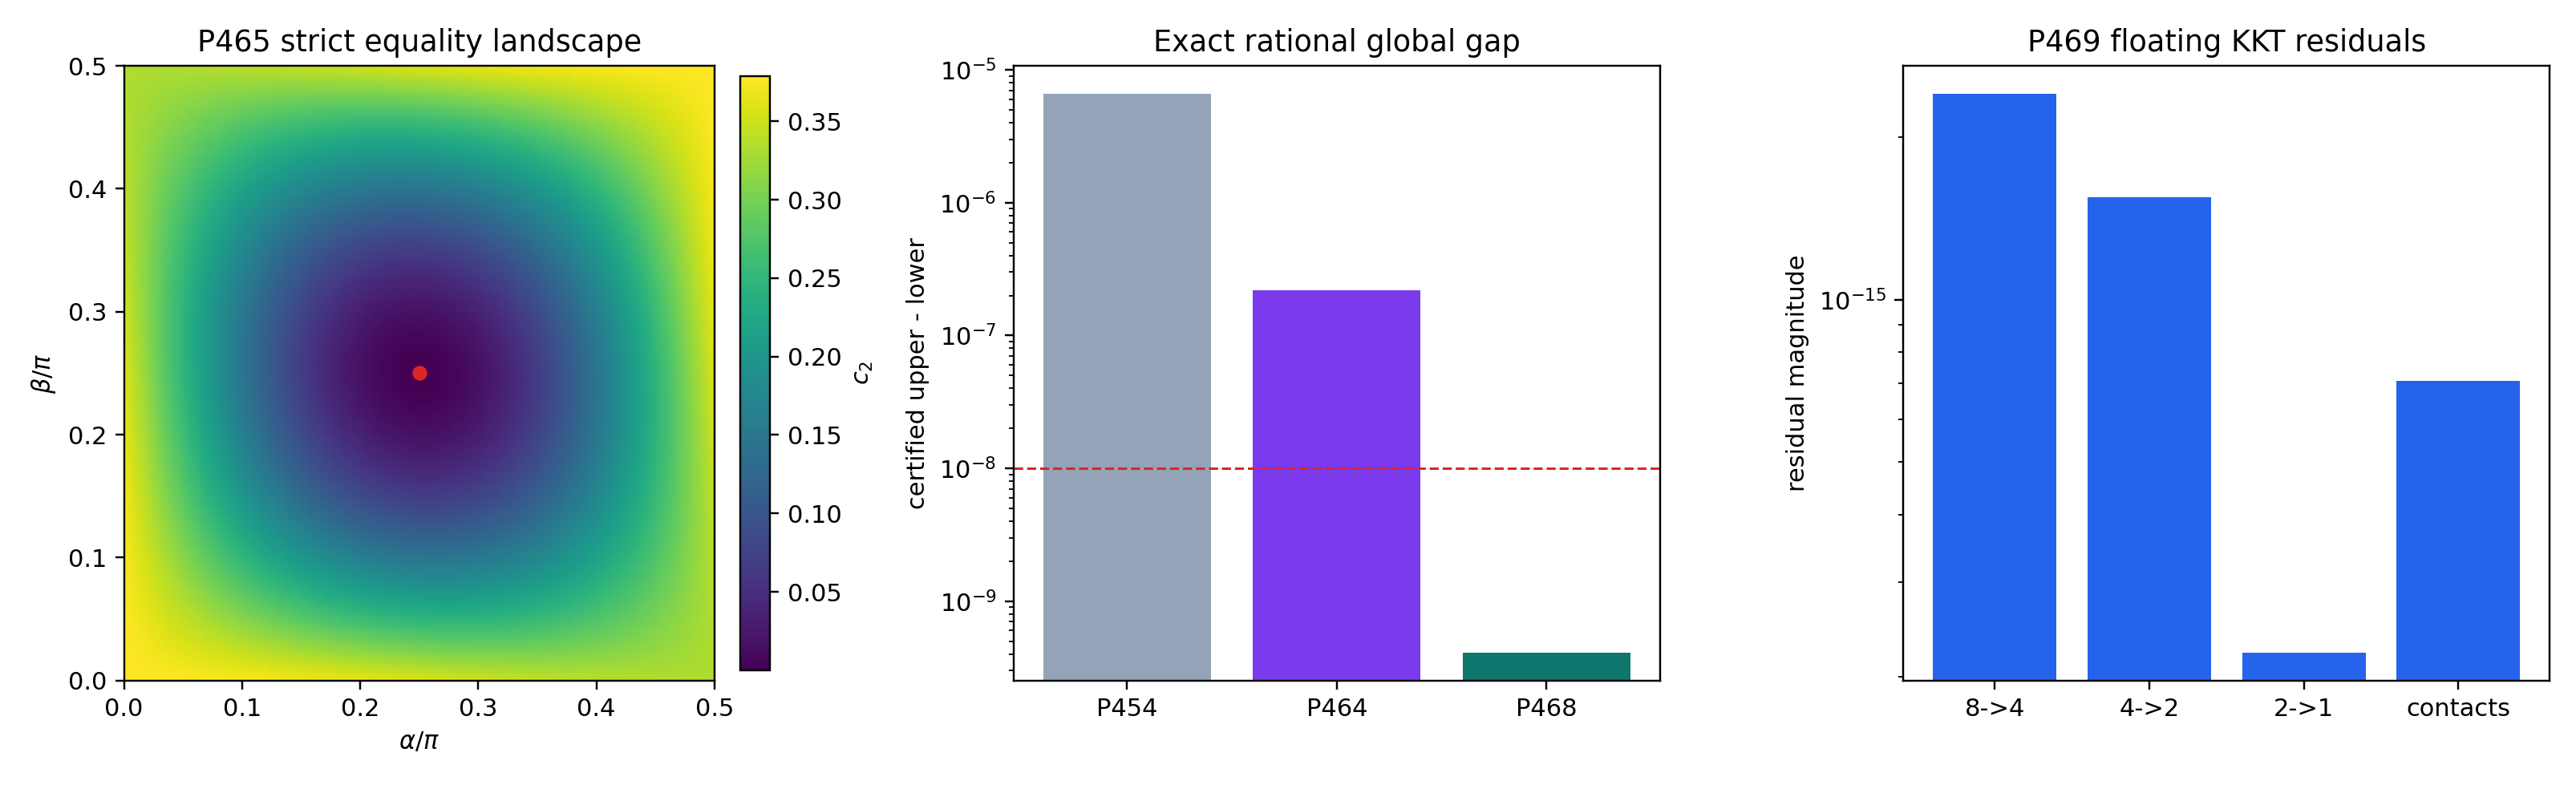
\includegraphics[width=0.97\textwidth]{FIN_Programs_465_468_469_Figures/p465_p468_p469_certificates.png}
\caption{Strict symmetrization equality, rational dual-gap collapse, and the floating full-ladder KKT residuals.}
\end{figure}

\chapter{Newly constructed objects}

\section{O176 --- Strict Reversal Equality Isolator}

\begin{center}
\begingroup\small
\setlength{\tabcolsep}{2.5pt}
\renewcommand{\arraystretch}{1.16}
\begin{longtable}{@{}p{0.420\textwidth}p{0.420\textwidth}@{}}
\toprule
\textbf{Field} & \textbf{Definition} \\
\midrule
\endhead
Domain & Complete declared four-sector probability simplex \\
Map & \(p\mapsto F((p+Rp)/2)-F(p)\) \\
Structure & Exact nonnegative coefficient factorization plus singular-face completion \\
Generated theorem & Zero set equals the palindromic fixed set \\
What it closes & Asymmetric co-optimizer loophole in P458 \\
What it does not close & Adaptive-channel or physical uniqueness \\
Confidence & \statusProven{} \\
\bottomrule
\end{longtable}
\endgroup
\end{center}

\section{O177 --- Interior Comb Support Ladder}

\begin{center}
\begingroup\small
\setlength{\tabcolsep}{2.5pt}
\renewcommand{\arraystretch}{1.16}
\begin{longtable}{@{}p{0.420\textwidth}p{0.420\textwidth}@{}}
\toprule
\textbf{Field} & \textbf{Definition} \\
\midrule
\endhead
Input & Positive ordered-comb normalizer \(N\) and Hermitian \(\Delta\) with nonsingular \(N^{1/2}\Delta N^{1/2}\) \\
Top operator & \(X_3(N)=N^{-1/2}|N^{1/2}\Delta N^{1/2}|N^{-1/2}/2\) \\
Lower equations & Equality of both principal blocks at every causal level \\
Mathematical role & Necessary and, with exact feasibility, sufficient KKT closure for an interior optimum \\
Current status & Exact construction and necessity theorem; exact O167 root open \\
Confidence & \statusProven{} structure; \statusStrong{} O167 root \\
\bottomrule
\end{longtable}
\endgroup
\end{center}

\section{O178 --- Support-Ladder Rational Closure Tube}

\begin{center}
\begingroup\small
\setlength{\tabcolsep}{2.5pt}
\renewcommand{\arraystretch}{1.16}
\begin{longtable}{@{}p{0.420\textwidth}p{0.420\textwidth}@{}}
\toprule
\textbf{Field} & \textbf{Definition} \\
\midrule
\endhead
Input & Floating O177 locator, rationalization scale, positive level shifts \\
Output & Strictly feasible rational nested dual or rejection \\
Admission rule & Exact Sylvester positivity plus complete operator perturbation payment \\
Generated theorem & Global upper \(0.52332810067104088\) \\
Failure mode prevented & Treating a near-KKT floating matrix as a dual theorem \\
Confidence & \textcolor{fingreen}{[Computer-assisted proof]} \\
\bottomrule
\end{longtable}
\endgroup
\end{center}

\chapter{Falsification and methodological audit}

\section{P465 attacks}

\begin{itemize}
\item 
The proof does not assume that the P452 quadratic coefficient is strictly positive everywhere; it classifies its exact zero.

\item 
It treats \(X=0\) and \(Y=0\) separately, avoiding division by \(Y\).

\item 
The \(Y=0\) face exposes a real blindness of \(D_2\); the independent \(D_3\) term repairs it.

\item 
The random scan is explicitly non-probative and cannot replace the algebra.

\end{itemize}

\section{P469 attacks}

\begin{itemize}
\item 
The support operator is derived from trace-norm duality, not guessed from the O167 pattern.

\item 
Full causal block equalities are tested, not only three face derivatives.

\item 
Positivity of the primal cascade and the spectral gap of \(H\) are checked.

\item 
Binary64 residuals are not promoted to an exact-root theorem.

\item 
The small signed support gap is identified as roundoff at a not-exactly feasible averaged ladder, not reported as a physical effect.

\end{itemize}

\section{P468 attacks}

\begin{itemize}
\item 
Every floating candidate is rejected unless all eight exact dual slacks pass.

\item 
The trigonometric matrix is not treated as rational; its enclosure radius is paid in operator norm.

\item 
\(\lambda\) is rounded upward.

\item 
The smallest admitted margin remains positive after perturbation.

\item 
The inherited primal lower bound is retained rather than replaced by the higher but uncertified floating O167 value.

\end{itemize}

\section{Claims deliberately rejected}

The following inferences remain invalid:

\begin{itemize}
\item 
residual \(10^{-15}\) implies exact O167 globality;

\item 
gap \(4.1\times10^{-10}\) may be declared zero;

\item 
unique mathematical code optimum implies a unique physical experiment;

\item 
an operational selector in a reduced discrimination problem discharges FIN's QW-2191 selector obstruction;

\item 
a dimensionless channel parameter supplies seconds, metres, energy, or action;

\item 
a downstream comb theorem completes the legacy-to-strict kernel bridge;

\item 
numerical or algebraic success constitutes laboratory confirmation.

\end{itemize}

\chapter{Interpretation for the present FIN state}

The current advance is operator-theoretic and operational. It strengthens the finite mathematical layer in two ways.

First, one complete declared information-loss optimization now has an exact symmetry equality theorem and a unique global probability law. This is a real uniqueness result inside a precisely specified finite model.

Second, the ordered-comb problem now has a canonical connection between a primal normalizer and the nested dual hierarchy. O177 shows that the apparent O167 pattern is not merely a convenient ansatz: it nearly satisfies the full-cone stationarity conditions generated by the trace-norm support. O178 then converts that insight into a rigorous global bracket without assuming the exactness of O167.

This does not solve the central FIN physics bridge. The result contains no physical clock, length, mass, action unit, preparation procedure, apparatus, environment, measurement record, or independent custody. It also leaves the strict selector and legacy-to-strict completion problems unchanged. Its scientific value is narrower and defensible: it replaces two numerical patterns by one exact uniqueness theorem, one exact rational global bound, and one sharply localized exact-root obligation.

\chapter{Ranked next research programs}

\begin{center}
\begingroup\small
\setlength{\tabcolsep}{2.5pt}
\renewcommand{\arraystretch}{1.16}
\begin{longtable}{@{}p{0.059\textwidth}p{0.104\textwidth}p{0.277\textwidth}p{0.419\textwidth}@{}}
\toprule
\textbf{Rank} & \textbf{Program} & \textbf{Question} & \textbf{Method and success criterion} \\
\midrule
\endhead
1 & P471 & Is there a unique exact O167 support-ladder root near the P469 point? & Select three independent equations; certify interval Jacobian nonsingularity and a Krawczyk inclusion \\
2 & P472 & Can \(N^{-1/2}|N^{1/2}\Delta N^{1/2}|N^{-1/2}\) be enclosed outward on a parameter box? & Spectral-gap-preserving polynomial, contour, or verified eigenspace calculus \\
3 & P473 & Does an exact P471 root produce a feasible zero-shift dual and exact global attainment? & Interval PSD and exact complementarity at all causal levels \\
4 & P474 & If P473 succeeds, is the full ordered-comb optimizer unique? & Strict complementarity, primal nondegeneracy, and tangent-cone kernel test \\
5 & P475 & Can the certified primal lower be improved to the rationalized O167 value? & Rational normalizer plus exact characteristic-polynomial trace-norm enclosure \\
6 & P461 & Formalize P452/\allowbreak{}P465 finite algebra & Lean proof of coefficient positivity and boundary equality cases \\
7 & P467 & Does O177 generalize to arbitrary slot number? & Inductive primal/\allowbreak{}dual comb ladder and interior complementarity theorem \\
8 & P466 & Does causal coherence advantage persist at four slots? & Symmetry-reduced four-slot witness plus exact rational admission \\
9 & P460 & Is O174 allocation stable under alternative admissible loss geometries? & Quotient sensitivity and ordering-margin theorem \\
10 & P470 & Which local operational conclusions persist under strict-kernel parameter boxes? & Interval perturbation audit with no legacy role transfer \\
11 & P463 & What is the minimal preparation/\allowbreak{}instrument contract needed to interpret the finite operators physically? & Typed operational interface, explicitly conditional and non-empirical \\
12 & P476 & Can the coarse-erasure uniqueness theorem be extended beyond the exact P452 parameter point? & Certified \((q,\theta)\)-region where \(4q^2\cos^2\theta>1\) and all boundary weights remain positive \\
\bottomrule
\end{longtable}
\endgroup
\end{center}

The next bounded batch is

\[
\boxed{P471\longrightarrow P472\longrightarrow P473}.
\]

If verified matrix functional calculus cannot be constructed locally within a finite budget, the batch must stop with a precise obstruction report rather than treating high-precision floating arithmetic as proof.

\chapter{Artifact list and restart}

\begin{itemize}
\item 
FIN\_Programs\_465\_468\_469\_Results.json

\item 
FIN\_Programs\_465\_468\_469\_Summary.csv

\item 
FIN\_Programs\_465\_468\_469\_P465\_Strict\_Symmetrization.csv

\item 
FIN\_Programs\_465\_468\_469\_P468\_Dual\_Refinement.csv

\item 
FIN\_Programs\_465\_468\_469\_P468\_Rational\_Dual.npz

\item 
FIN\_Programs\_465\_468\_469\_P469\_Nested\_KKT.csv

\item 
FIN\_Programs\_465\_468\_469\_Figures/\allowbreak{}p465\_p468\_p469\_certificates.png

\item 
fin\_programs\_465\_468\_469.py

\item 
test\_fin\_programs\_465\_468\_469.py

\end{itemize}

Recompute with:

\begin{Verbatim}[fontsize=\small]
MPLCONFIGDIR=/tmp/fin-mpl-1043 python3 fin_programs_465_468_469.py
python3 -m unittest -v test_fin_programs_465_468_469.py
python3 fin_programs_465_468_469_to_latex.py
lualatex -interaction=nonstopmode -halt-on-error \
  FIN_Local_Research_Checkpoint_P465_P469_EN.tex
sha256sum -c FIN_PROGRAMS_465_468_469_RELEASE_MANIFEST.sha256
\end{Verbatim}

\chapter{Conclusion}

Release 10.43 closes one genuine uniqueness problem and nearly closes one global semidefinite optimization problem without hiding the remaining logical gap. The declared coarse-erasure probability law is now unique on its complete simplex. The three-slot ordered-comb value is globally confined to an interval of width \(4.1055151\times10^{-10}\), and the O167 candidate satisfies the full nested KKT equations to machine precision. Exact O167 attainment remains open until a verified nonlinear root and zero-shift dual are constructed.

The deepest surviving interpretation remains mathematical: FIN currently contains a disciplined finite operator and information-processing framework with increasingly sharp uniqueness, duality, and causal-comb certificates. It does not yet contain the selector, dimensional conversion, operational preparation, or empirical record required to become experimentally testable physics.


\clearpage\chapter*{Reproduction certificate}
\addcontentsline{toc}{chapter}{Reproduction certificate}
\begin{Verbatim}[fontsize=\small]
MPLCONFIGDIR=/tmp/fin-mpl-1043 \
python3 fin_programs_465_468_469.py
python3 -m unittest -v \
  test_fin_programs_465_468_469.py \
  test_fin_checkpoint_p465_p469.py
python3 fin_programs_465_468_469_to_latex.py
lualatex -interaction=nonstopmode -halt-on-error \
  FIN_Local_Research_Checkpoint_P465_P469_EN.tex
sha256sum -c FIN_PROGRAMS_465_468_469_RELEASE_MANIFEST.sha256
\end{Verbatim}
\noindent\textbf{Suggested citation:}
\.Zuchowski, K. (2026). \emph{FIN Local Research Checkpoint P465--P469:
Strict Full-Simplex Uniqueness and a Support-Ladder Rational Dual Certificate}
(Release 10.43; Version 1.0.0) [Preprint].
\end{document}
